\section{Appendix}
\subsection{Personas}

\begin{figure}[h!]
  \centering
  \subfloat[Jeff and Judy Seavers]{\label{fig:seavers}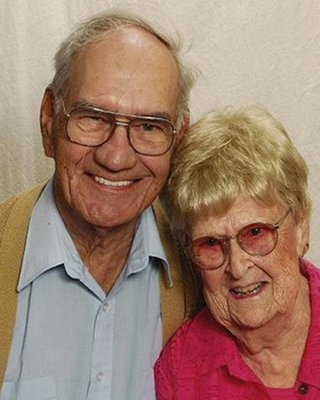
\includegraphics[width=0.3\textwidth]{Images/jeff_and_judy_seavers.jpg}}                
  \subfloat[Sarah Gordon]{\label{fig:gordon}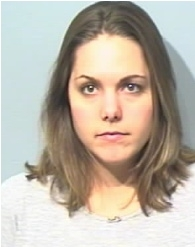
\includegraphics[width=0.3\textwidth]{Images/sarah_gordon.jpg}}
  \subfloat[Bruce Walker]{\label{fig:walker}
\includegraphics[width=0.3\textwidth]{Images/bruce_walker.jpg}}
  \caption{Personas}
  \label{fig:personas}
\end{figure}

\subsection{User Involvement Methods}
\subsubsection{Accompanying letter}\label{sec:letter}
Dear \dots

For our course ``Human Computer Interaction'', we have to design a system for selling baby clothes. Our group decided to build a web-based system, for which we need your help. In order to find out about which features our system should include, we made a questionnaire with some questions concerning web shops (in general and clothes/baby clothes in particular).
If you can spare fifteen minutes of your time, we'd greatly appreciate if you could help us and fill out the questions.

Thank you very much!\\
Alban Edouard, Gianin Basler, Irem Tanriseven, Joana Welti


\subsubsection{Questionnaires}

Why the Prototype files appear before the questionnaires ???

\begin{figure}[h!]
\centering
\includegraphics[width=1.0\textwidth]{User_Involvement_Methods/Questionnaires/Questionnaire_Web_Shops_v2.pdf}
\end{figure}

\begin{figure*}[h!]
\centering
\includegraphics[width=1.0\textwidth]{User_Involvement_Methods/Questionnaires/Questionnaire_Web_Shops_v2_2.pdf}
\caption{Questionnaire First Draft}
\label{fig:draft}
\end{figure*}


\begin{figure*}[h!]
\centering
\includegraphics[width=1.0\textwidth]{User_Involvement_Methods/Questionnaires/Questionnaire_Web_Shops_v3.pdf}
\end{figure*}

\begin{figure*}[h!]
\centering
\includegraphics[width=1.0\textwidth]{User_Involvement_Methods/Questionnaires/Questionnaire_Web_Shops_v3_2.pdf}
\caption{Questionnaire Final Version}
\label{fig:final}
\end{figure*}

\subsubsection{Prototype}
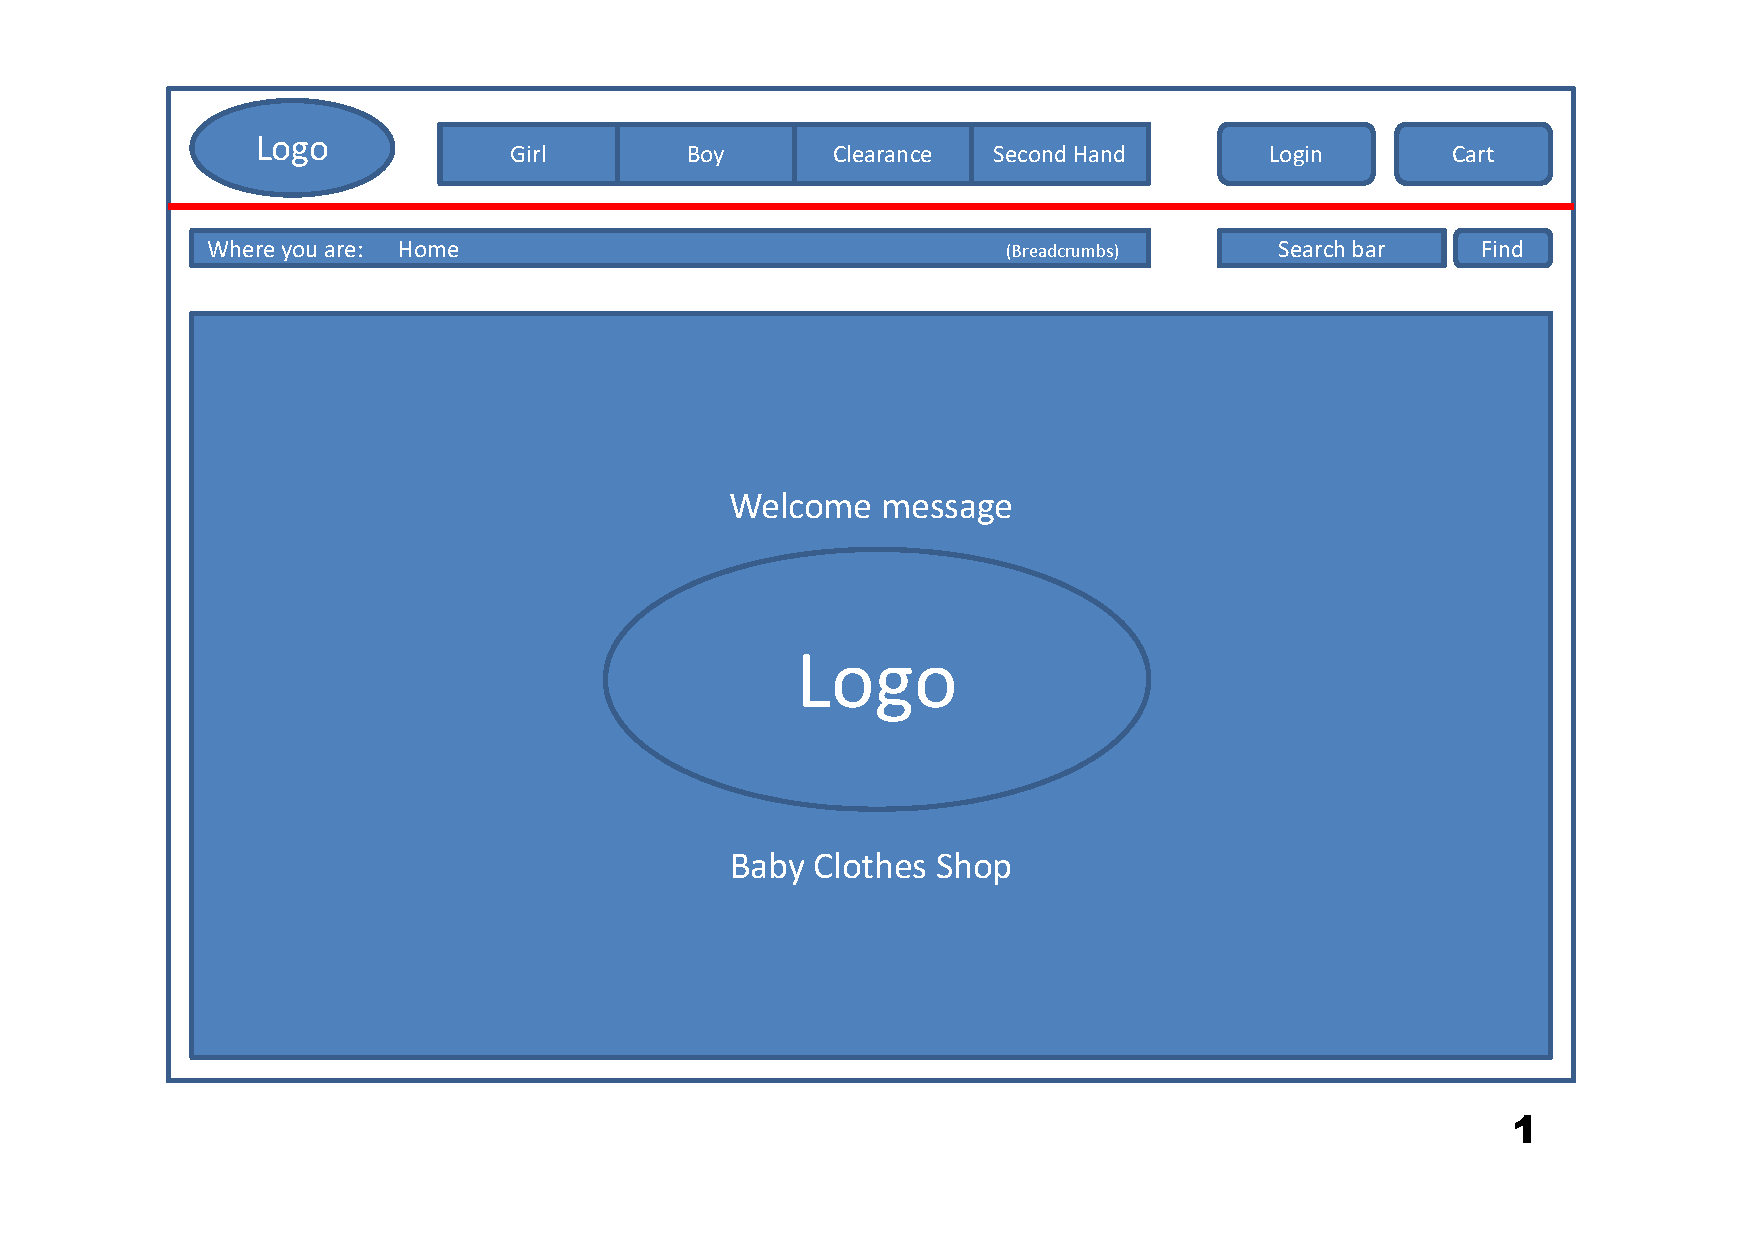
\includepdf[pages=-]{Prototype/HCI_Prototype_2.pdf}
